\documentclass[10pt, letterpaper]{article}

\usepackage{amssymb,amsmath,amsfonts,eurosym,geometry,ulem,graphicx,caption,color,setspace,sectsty,comment,footmisc,caption,natbib,pdflscape,subfigure,array,hyperref}
\usepackage{xcolor}
\usepackage{mathptmx}
\usepackage{listings}
\lstset{language=Matlab}
\hypersetup{
    colorlinks,
    linkcolor={red!50!black},
    citecolor={blue!50!black},
    urlcolor={blue!80!black}
}
\normalem
\usepackage[flushleft]{threeparttable}
    
\onehalfspacing
\newtheorem{theorem}{Theorem}
\newtheorem{corollary}[theorem]{Corollary}
\newtheorem{proposition}{Proposition}
\newenvironment{proof}[1][Proof]{\noindent\textbf{#1.} }{\ \rule{0.5em}{0.5em}}

\newtheorem{hyp}{Hypothesis}
\newtheorem{subhyp}{Hypothesis}[hyp]
\newtheorem{asu}{Assumption}
\renewcommand{\thesubhyp}{\thehyp\alph{subhyp}}

\newcommand{\red}[1]{{\color{red} #1}}
\newcommand{\blue}[1]{{\color{blue} #1}}

\newcolumntype{L}[1]{>{\raggedright\let\newline\\arraybackslash\hspace{0pt}}m{#1}}
\newcolumntype{C}[1]{>{\centering\let\newline\\arraybackslash\hspace{0pt}}m{#1}}
\newcolumntype{R}[1]{>{\raggedleft\let\newline\\arraybackslash\hspace{0pt}}m{#1}}

\geometry{left=1.0in,right=1.0in,top=1.0in,bottom=1.0in}

\begin{document}

\title{Homework 1: ECON512}
\author{Joonkyo Hong}
\date{}
\maketitle
\smallskip

\noindent 1. The associated graph are depicted below.

\begin{figure}[!h]
\begin{center}
  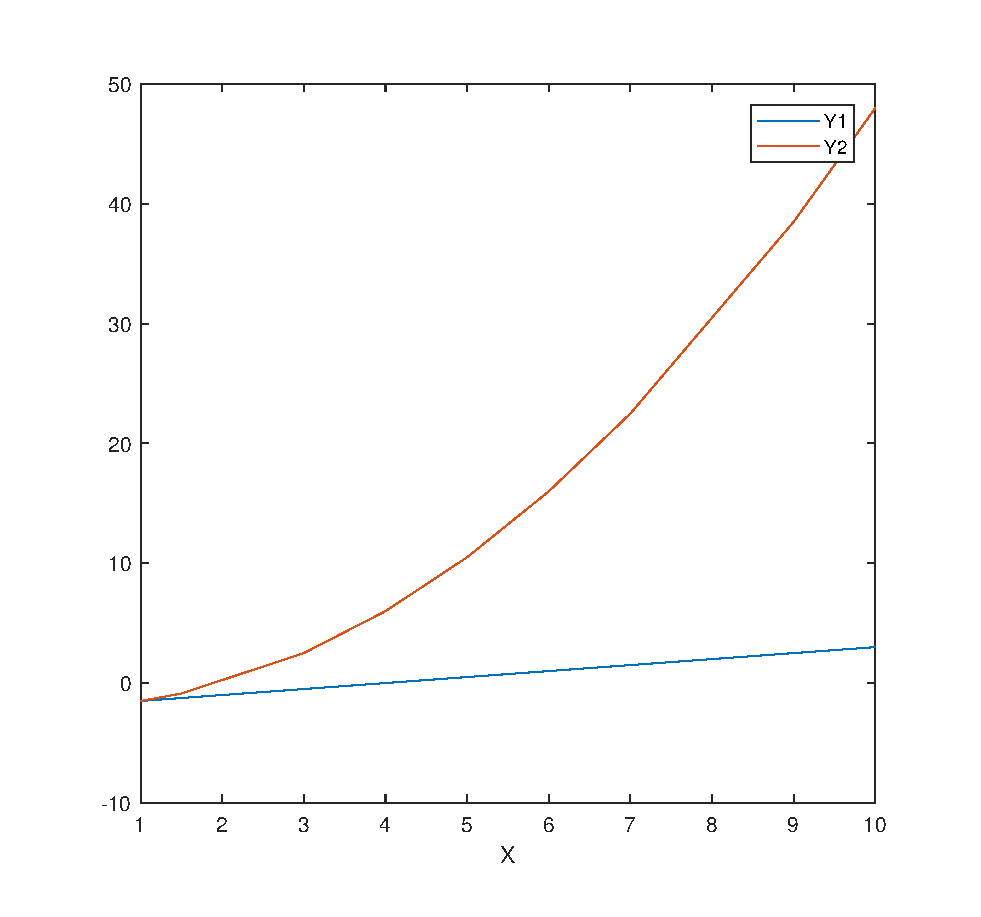
\includegraphics[width=0.4\linewidth]{graph1.eps}
  \caption{}
  \label{fig:graph}
\end{center}
\end{figure}

\noindent 2. Summation is 1000.

\noindent 3. Here are the results 
\begin{align}
C & = \begin{bmatrix}
         29 \\ 133 \\ 43
      \end{bmatrix}    \nonumber \\
D & = \begin{bmatrix}
        -3.2505 \\ 0.3961 \\ 0.8037 
       \end{bmatrix}    \nonumber \\
E & = b A' \iota = 200, \text{where $\iota$ is a vector which all elements are one} \nonumber \\
F & = \begin{bmatrix}
          2 & 4 \\
          3 & 12 
      \end{bmatrix} \nonumber \\
x & = A^{-1}b = \begin{bmatrix}
                  -0.1622 \\ 1.2432 \\ -1.1081
                 \end{bmatrix} \nonumber 
\end{align}

\noindent 4. This is nothing but $B = I_{5} \otimes A$

\noindent 5. With seed 2, the following result arises. 
\begin{align}
A & = \begin{bmatrix}
          0 & 0 & 1 \\
          0 & 0 & 1 \\
          1 & 1 & 0 \\
          0 & 0 & 1 \\
          0 & 0 & 0 
       \end{bmatrix} \nonumber
\end{align} 

\noindent 6. Let
\begin{align}
y_{i}& = \begin{bmatrix}
           prod_{i1} \\
           prod_{i2} \\
           \vdots    \\
           prod_{iT}
         \end{bmatrix}, \nonumber \\          
x_{i}^{'}& = \begin{bmatrix}
           1 & Export_{i1} & RD_{i1} & cap_{i1} \\
           1 & Export_{i2} & RD_{i2} & cap_{i2} \\
           \vdots &  \vdots & \vdots & \vdots   \\
           1 & Export_{iT} & RD_{iT} & cap_{iT}
          \end{bmatrix}. \nonumber 
\end{align}
Then, OLS estimator $\hat{\beta}$ is computed by 
\begin{align}
\hat{\beta} = \big( \sum_{i} x_{i} x_{i}' \big)^{-1} \big( \sum_{i} x_{i} y_{i} \big), \nonumber
\end{align}
and the corresponding standard errors are squared root of the diagonal components in the following matrix:
\begin{align}
\big( \sum_{i} x_{i} x_{i}' \big)^{-1} \big( \sum x_{i}\hat{e}_{i}\hat{e}_{i}^{'}x_{i}^{'} \big) \big( \sum_{i} x_{i} x_{i}' \big)^{-1}, \nonumber
\end{align}
where
\begin{align}
\hat{e}_{i} = y_{i} - x_{i}^{'}\hat{\beta}. \nonumber
\end{align}
Table \ref{tab:1} reports the estimates and relevant standard errors.


\begin{table}[!h]
  \begin{center}
    \caption{Estimation Results}  
    \label{tab:1}
    \begin{tabular}{c|c} % <-- Alignments: 1st column left, 2nd middle and 3rd right, with vertical lines in between
      \hline\hline
                                                                      &    \textbf{Dep: Productivity}  \\
      \hline    
      Exporters                                                         &  $ 0.1210^{***}    $   \\
                                                                        &  $\big( 0.009 \big)$    \\      
      R \& D                                                            &  $  0.1399^{***}   $   \\
                                                                        &  $\big( 0.0138 \big)$    \\      
      Capitals                                                          &  $  0.0295^{***}   $    \\
                                                                        &  $\big( 0.004 \big)$    \\     
      Constant                                                          &  $  0.0817^{***}  $  \\
                                                                        &  $\big( 0.0345 \big)$  \\                                                                              
      \hline
    \end{tabular}
  \end{center}
  \begin{tablenotes}
      \item {\footnotesize \it The table displays estimation results of the the model. Dependent variable is productivity of a firm in a certain wave. Standard errors are in parenthesis. Asterisks mark rejection at the 1\% (***).}
   \end{tablenotes}
\end{table} 

\clearpage

\begin{verbatim}

%%%%%%%%%%%%%%%%%%%%%%%%%%%%%%%%%%%%%%%%%%%%%%%%%%%%%%%%%%%
% Homework #1 ECON 512                                    %
% Written by Joonkyo (Jay) Hong, 31 Aug 2018              %
%%%%%%%%%%%%%%%%%%%%%%%%%%%%%%%%%%%%%%%%%%%%%%%%%%%%%%%%%%%

%% Problem 1.

X = [1 1.5 3 4 5 6 7 9 10];
Y1 = -2 + .5*X;
Y2 = -2 + .5*X.^2;

figure(1)
plot(X,[Y1; Y2]);
legend("Y1","Y2");
xlabel("X");

%% Problem 2

vec_problem2 = linspace(-10,20,200);
vec_problem2 = vec_problem2';
ans_problem2 = sum(vec_problem2);
ans_problem2

%% Problem 3

A = [2 4 6;
     1 7 5;
     3 12 4];
b = [-2;3;10];

C = A'*b
D = (A'*A)\b
E = b'*A*[1;1;1]
F = A;
F(:,3)=[];
F(2,:)=[];
F
x = A\b

%% Problem 4

B = kron(eye(5),A)

%% Problem 5

rng(2);
matrix_problem5 = normrnd(10,5,5,3);
ans_problem5 = matrix_problem5;
ans_problem5(ans_problem5<10)=0;
ans_problem5(ans_problem5>=10)=1;
ans_problem5


%% Problem 6

dataset = csvread('datahw1.csv',0,0);

ymat = (dataset(:,5));
xmat = [ones(length(ymat),1) dataset(:,3:4) (dataset(:,6))];

ols_est = xmat'*xmat\xmat'*ymat;
k = length(ols_est);
emat = ymat-xmat*ols_est;
wave = 4;
obs= length(ymat)/4;
center_sand = zeros(k,k);
for i=1:obs
    ei = emat((i-1)*wave+1:i*wave,1); xi = xmat((i-1)*wave+1:i*wave,:);
    center_sand = center_sand + xi'*ei*ei'*xi;
end

ols_cov = (xmat'*xmat)\center_sand/(xmat'*xmat);
ols_se = sqrt(diag(ols_cov));

 disp("              ");
 disp("OLS estimates in Problem 6");
 disp("Parameter Estimates and Standard Errors");
 disp(" beta0        beta1       beta2      beta3");
 disp(num2str(ols_est'));
 disp(num2str(ols_se'));
 
\end{verbatim}
                     

\end{document}